\documentclass{standalone}
\usepackage{tikz-network}

\begin{document}
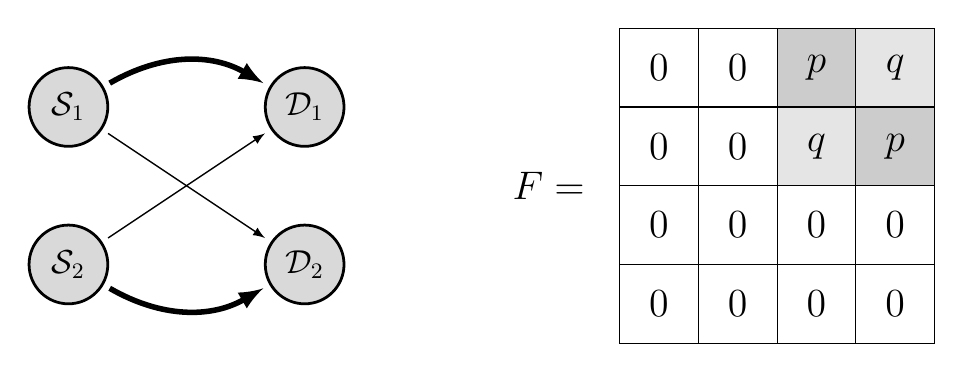
\begin{tikzpicture}

\SetVertexStyle[LineWidth=1, FillColor=black!15!white, LineColor=black, OuterSep=3, TextFont=\large]
\SetEdgeStyle[Color=black]
\SetTextStyle[TextFont=\Large]

\Vertex[x=-1,label=$\mathcal{S}_1$,size=1]{1}
\Vertex[x=-1,y=-2,label=$\mathcal{S}_2$,size=1]{2}
\Vertex[x=2,label=$\mathcal{D}_1$,size=1]{3}
\Vertex[x=2,y=-2,label=$\mathcal{D}_2$,size=1]{4}

\Edge[Direct,lw=2,bend=30,position={above=0.1},fontscale=2](1)(3)
\Edge[Direct,lw=2,bend=-30,position={below=0.1},fontscale=2](2)(4)
\Edge[Direct,lw=0.5,position={left=0.1},fontscale=2](1)(4)
\Edge[Direct,lw=0.5,position={right=0.1},fontscale=2](2)(3)

\Text[x=5.1,y=-1]{$F = $}

\draw[fill=black!20!white] (8,0) rectangle ++(1,1);
\draw[fill=black!10!white] (9,0) rectangle ++(1,1);
\draw[fill=black!10!white] (8,-1) rectangle ++(1,1);
\draw[fill=black!20!white] (9,-1) rectangle ++(1,1);
\draw[fill=white] (6,0) rectangle ++(1,1);
\draw[fill=white] (7,0) rectangle ++(1,1);
\draw[fill=white] (6,-1) rectangle ++(1,1);
\draw[fill=white] (7,-1) rectangle ++(1,1);
\draw[fill=white] (6,-2) rectangle ++(1,1);
\draw[fill=white] (7,-2) rectangle ++(1,1);
\draw[fill=white] (6,-3) rectangle ++(1,1);
\draw[fill=white] (7,-3) rectangle ++(1,1);
\draw[fill=white] (8,-2) rectangle ++(1,1);
\draw[fill=white] (9,-2) rectangle ++(1,1);
\draw[fill=white] (8,-3) rectangle ++(1,1);
\draw[fill=white] (9,-3) rectangle ++(1,1);

\Text[x=8.5,y=0.5]{$p$}
\Text[x=9.5,y=0.5]{$q$}
\Text[x=8.5,y=-0.5]{$q$}
\Text[x=9.5,y=-0.5]{$p$}

\Text[x=6.5,y=0.5]{$0$}
\Text[x=6.5,y=-0.5]{$0$}
\Text[x=6.5,y=-1.5]{$0$}
\Text[x=6.5,y=-2.5]{$0$}

\Text[x=7.5,y=0.5]{$0$}
\Text[x=7.5,y=-0.5]{$0$}
\Text[x=7.5,y=-1.5]{$0$}
\Text[x=7.5,y=-2.5]{$0$}

\Text[x=8.5,y=-1.5]{$0$}
\Text[x=8.5,y=-2.5]{$0$}

\Text[x=9.5,y=-1.5]{$0$}
\Text[x=9.5,y=-2.5]{$0$}

\end{tikzpicture}
\end{document}